\section{From existing methods to the approach}\label{sec:approach}

Several research traditions each solve part of the problem. None answers the question this project
asks: \emph{in this domain, where does the written record stop, and what kind of knowledge is likely
to lie beyond it?} This section first states the approach, then what each tradition contributes to
it, then the closest prior work.

\subsection{The central model}\label{sec:approach-model}

\Cref{fig:model} shows the approach. Steps 1--6 are built in the PoC; steps 7--9 are not.

\begin{figure}[tbp]
  \centering
  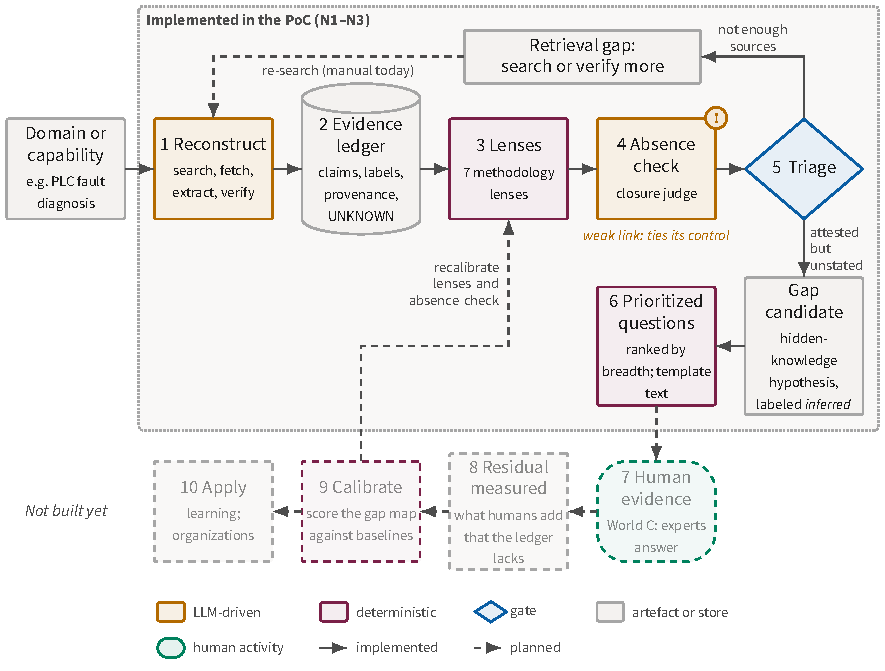
\includegraphics{figures/pdf/fig02_model.pdf}
  \caption[The central model]{What is the whole approach, and which parts exist today? Steps 1--6
    (solid) are implemented in the PoC; steps 7--9 (dashed) are future work. Triage splits the output
    into retrieval gaps, listed for further search, and gap candidates, which become hypotheses
    labeled \emph{inferred} and expert questions. The absence check (step~4) is the weak link.}
  \label{fig:model}
\end{figure}

\begin{description}[style=nextline, leftmargin=1.5em, itemsep=1pt, topsep=2pt]
  \item[1--2 Reconstruct into an evidence ledger] Fetch public sources, extract claims, locate each
    quote in a hashed snapshot, and verify it with a model of another family. Each claim carries one
    of six epistemic labels; \code{unknown} marks a slot searched and not covered.
  \item[3 Lenses] Seven lenses \emph{fire} when sources attest a construct but not its content, for
    example rival causes with no sign that separates them.
  \item[4 Absence check] A judge reads the sentences a lexical retriever pulls from the ledger (up to
    8 verified and 4 unverified per probe) and returns \emph{closed}, \emph{partial} or \emph{open};
    closed firings are dropped.
  \item[5 Triage] A \textbf{retrieval gap} (nothing found, one independent source, unverified text
    only, answered by a sibling run, or an unreadable verdict) calls for more search, not an expert.
    A \textbf{gap candidate} has at least two independent sources and an element the absence check
    did not find fully stated. It becomes a hidden-knowledge hypothesis labeled \code{inferred}.
  \item[6 Questions] Template-filled (no model writes them), with a predicted knowledge type and a
    human channel; ranked by a breadth rubric, not by expected information gain.
  \item[7--9 Future] Expert answers measure the residual, score and recalibrate the gap map, and only
    then feed instruction or organizational uses.
\end{description}
\evhyp{} If a lens fires, a working absence check does not find the missing element, and the attested
side has broad support, then practitioners are more likely there than elsewhere to hold knowledge the
text lacks. The PoC builds the mechanism; it does not test this hypothesis.


\subsection{What each tradition contributes}\label{sec:traditions}

\Cref{fig:lenses} shows which research tradition gives which lens, the missing element each lens looks
for, and the human channel that would ask about it. \evlit{} The traditions differ in strength. That
experts omit decisions, cues and interpretations is established in direction, from small studies in
single domains (\cref{sec:problem}). CTA-based instruction beats other ways of choosing training
content in a meta-analysis of few studies ($g = 0.871$; \cite{tofelgrehl2013cognitive}). The Critical
Decision Method, PARI, Evidence-Centered Design and knowledge components are established methods
\parencite{klein1989critical,hall1995procedural,mislevy2003structure,koedinger2012knowledge}. Causal
ambiguity rests on one large study of 271 observations \parencite{szulanski1996exploring}; the tacit
knowledge typology is conceptual, not empirical \parencite{polanyi1966tacit,collins2010tacit}; and
reporting bias is shown for commonsense facts, not measured in expert text
\parencite{gordon2013reporting}. \evint{} The literature therefore supports the \emph{constructs} the
lenses use. It does not support the lenses: no cited study tests whether a detector built on these
constructs finds real expert knowledge in text (Extended Technical Report, Section~3). Every mapping from
a construct to a lens is our interpretation, and every lens output carries the label \code{inferred}.

\begin{figure}[tbp]
  \centering
  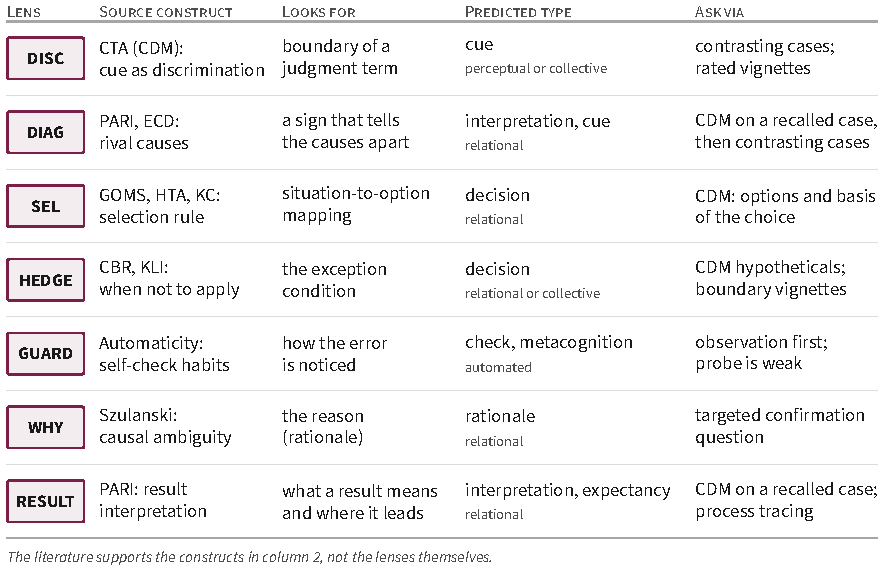
\includegraphics{figures/pdf/fig03_lenses.pdf}
  \caption[Which methodology gives which lens]{Which research method gives which methodology lens,
    what missing element each lens looks for, its predicted knowledge type, and the human channel
    that would ask about it. None of the lenses has been validated against a human judgment of where
    expert knowledge is missing.}
  \label{fig:lenses}
\end{figure}

\subsection{Closest prior work, and what may be new}\label{sec:novelty}

\evlit{} Our search, to September 2026, found precedent for every step. \textcite{torre2020ai} check
GDPR privacy policies for content types that a conceptual model of the regulation requires; on 24
unseen policies they found 45 of 47 incompleteness issues. That is typed absence detection in one of
our own domains, but the reference fixes in advance what should be present.
\textcite{anthonio2022clarifying} find underspecified phrases in instructional text, with later human
edits as gold. DRMiner mines design rationale from issue trackers \parencite{zhao2024drminer}.
\textcite{luitel2024improving} flag terms missing from requirements, and OntoAgent picks interview
questions from an ontology \parencite{jin2026chat}. \evint{} Each works on one document or interview
against a reference that already contains the missing content. None predicts what practitioners know
beyond all written sources, or routes a gap to an elicitation channel. \Cref{tab:novelty} places the
main elements.

\begin{table}[htbp]
  \centering\footnotesize
  \caption[Novelty ledger]{Condensed novelty ledger; the full ledger is in the Extended Technical Report, Section~4.3. \emph{Adaptation}: a known
    idea on a new unit or purpose.}
  \label{tab:novelty}
  \begin{tabularx}{\linewidth}{@{}>{\raggedright\arraybackslash}p{0.34\linewidth}
      >{\raggedright\arraybackslash}p{0.2\linewidth}>{\raggedright\arraybackslash}X@{}}
    \toprule
    Element & Category & Precedent or reason \\
    \midrule
    Claim ledger: verbatim spans from hashed snapshots, verifier of another family & Known
      combination & \textcite{min2023factscore,rashkin2023measuring} \\
    \code{unknown} only for a searched, uncovered slot & Adaptation & Abstention and completeness
      \parencite{razniewski2024completeness} \\
    Methodology lenses as absence detectors & Adaptation & Typed absence detection exists
      \parencite{torre2020ai,anthonio2022clarifying}; new here only the source of the types and the
      target. Validity not shown \\
    Knowledge type and elicitation channel per candidate & Adaptation / known method & Taxonomies and
      channel choice exist \parencite{collins2010tacit,klein1989critical} \\
    Retrieval gaps routed to search, not to experts & Adaptation & Retrieve-or-ask split in
      \textcite{taranukhin2026infogatherer} \\
    Synthetic output as predictor only, never criterion & Known method & Limits of simulated samples
      \parencite{bisbee2024synthetic} \\
    Scoring a gap map against published CTA results & Potentially novel (uncertain) & No such
      comparison found; gold sets are small \\
    Whole chain, domain-neutral, evidence status carried end to end & Potentially novel (uncertain) &
      No single system found; commercial tools may not publish methods \\
    \bottomrule
  \end{tabularx}
\end{table}

\evint{} The most defensible claim is the combination: a provenance ledger with an evidence status
per claim, expertise constructs as typed absence detectors, a knowledge type and channel per
suspected gap, and search failures kept apart from expert questions. It holds only as a proof of
concept. The evaluation design that scores a gap map against published CTA results is a stronger
novelty candidate than the system, but it has not run.
